\section{Auswertung}
\label{sec:Auswertung}
In der Auswertung wurden die Graphen mit Matplotlib \cite{matplotlib} und NumPy \cite{numpy} angefertigt.\\


Folgende Werte waren bereits vor der Messung bekannt:
\begin{displaymath}
R_1 = \SI{67.2(2)}{\ohm}
\end{displaymath}
\begin{displaymath}
R_2 = \SI{682(1)}{\ohm}
\end{displaymath}
\begin{displaymath}
L = \SI{16.78(9)e-3}{\henry}
\end{displaymath}
\begin{displaymath}
C = \SI{2.066(6)e-9}{\farad}
\end{displaymath}


\subsection{Bestimmung vom effektivem Widerstand}
%\begin{figure}[H]
%	\centering
%	\caption{Einhüllende.}
%	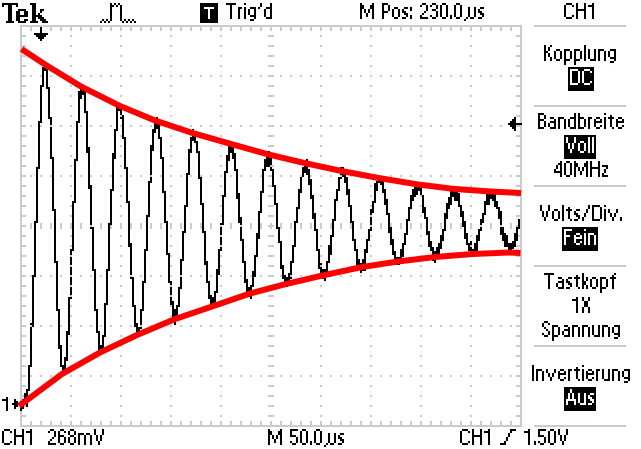
\includegraphics[width=\linewidth-70pt,height=\textheight-70pt,keepaspectratio]{content/Einhuellende.JPG}
%	\label{fig:graein}
%\end{figure}
\begin{figure}[H]
	\centering
	\caption{$A_C$ im $RCL$-Kreis in Abhängigkeit der Zeit.}
	\includegraphics[width=\linewidth-70pt,height=\textheight-70pt,keepaspectratio]{graa.pdf}
	\label{fig:graa}
\end{figure}
\input{../build/taba.tex}
Es gilt:
\begin{equation}
	U_C(t) = A_C \cdot e^{-\mu \cdot t} \cdot \cos(\omega_{res} \cdot t + \theta)\text{.}
\end{equation}
Es wird mithilfe einer nichtlinearen Ausgleichsrechnung der Form $y=a\cdot e^{-b t}$ mittels SciPy \cite{scipy} $\mu$ bestimmt. Es ergibt sich aus den Daten aus Tabelle 1 und Formel (21):
\begin{displaymath}
\mu = b = \SI{3.87(5)e3}{\per\second}\text{.}
\end{displaymath}
Hiermit ergibt sich für den effektiven Widerstand $R_{eff}$ durch die Formel (3):
\begin{displaymath}
R_{eff} = \SI{130 \pm 1.9}{\ohm}
\end{displaymath}
und mit der Formel (10):
\begin{displaymath}
\tau = \SI{2.582(34)e-4}{\second}\text{.}
\end{displaymath}


\subsection{Bestimmung des Widerstandes, bei welchem der aperiodische Grenzfall erreicht wird}
Beobachtet wurde der aperiodische Grenzfall bei
\begin{displaymath}
R_{ap} = \SI{272}{\ohm}\text{.}
\end{displaymath}
Mit den gegebenen Werten $L$ und $C$ errechnet sich jedoch mit Formel (2):
\begin{displaymath}
R_{ap} = \SI{5700(17)}{\ohm}\text{.}
\end{displaymath}
Die Abweichung zum errechnetem Wert liegt somit bei $\SI{5428(17)}{\ohm}$.
Diese starke Abweichung zwischen dem errechneten und gemessenen Wert muss in der Diskussion geklärt werden.


\subsection{Bestimmung der Güte q sowie der Resonanzbreite des RCL-Kreises}
\begin{figure}[H]
	\centering
	\caption{$A_C$ im angetriebenen $RCL$-Kreis in Abhängigkeit von $f_{\text{Antrieb}}$.}
	\includegraphics[width=\linewidth-70pt,height=\textheight-70pt,keepaspectratio]{grac1.pdf}
	\label{fig:grac1}
\end{figure}
Es werden mithilfe einer nichtlinearen Ausgleichsrechnung der Form $y=\frac{1}{\sqrt{(1-(2a\cdot x)^2)^2+(b\cdot x)^2}} $ mittels SciPy \cite{scipy} $LC$ und $RC$ bestimmt. Es ergibt sich aus den Daten aus Tabelle 2 und Formel (12):
\begin{displaymath}
LC = a^2 = \SI{3.626(13)e-11}{\second\squared}
\end{displaymath}
\begin{displaymath}
RC = b = \SI{1.505(12)e-6}{\ohm\squared\second}\text{.}
\end{displaymath}
Hiermit berechnet sich mit Formel (16):
\begin{displaymath}
q = \num{4.002(33)}\text{.}
\end{displaymath}
Mit den gegebenen Werten $R_2$, $C$ und $L$ ergibt sich mit Formel (16):
\begin{displaymath}
q = \num{4.179(14)}\text{.}
\end{displaymath}
Es lässt sich also eine systematische Abweichung  nach unten feststellen.


\begin{figure}[H]
	\centering
	\caption{Lineare Betrachtung von $A_C$ im nahen Bereich um $f_{res}$.}
	\includegraphics[width=\linewidth-70pt,height=\textheight-70pt,keepaspectratio]{grac2.pdf}
	\label{fig:grac2}
\end{figure}
\input{../build/tabc.tex}
Für die Breite der Ressonanzkurve $B$ ergibt sich mit dem zuvor bestimmten $LC$ und $RC$, der Formel (17) und der Beziehung $B = f_+ - f_- = \frac{\omega_+ - \omega_-}{2\pi}$:
\begin{displaymath}
B = f_+ - f_- = \SI{6.82(6)e3}{\per\second}\text{.}
\end{displaymath}
Mit den gegebenen Werten für $L$, $R_2$ und $C$ ergibt sich:
\begin{displaymath}
B = f_+ - f_- = \SI{6.66(4)e3}{\per\second}\text{.}
\end{displaymath}
Auch hier ist eine systematische Abweichung zwischen den aus den gegeben Werten und aus den gemessenen Werten errechneten Werten erkennbar.



\subsection{Untersuchung der Phasendifferenz in Abhängigkeit der Frequenz}
\begin{figure}[H]
	\centering
	\caption{Phase $\varphi$ im angetriebenen $RCL$-Kreis in Abhängigkeit von $f_{\text{Antrieb}}$ }
	\includegraphics[width=\linewidth-70pt,height=\textheight-70pt,keepaspectratio]{grad1.pdf}
	\label{fig:grad1}
\end{figure}
\begin{figure}[H]
	\centering
	\caption{Lineare Betrachtung von $\varphi$ im nahen Bereich um $f_{res}$}
	\includegraphics[width=\linewidth-70pt,height=\textheight-70pt,keepaspectratio]{grad2.pdf}
	\label{fig:grad2}
\end{figure}
\input{../build/tabd.tex}
\newpage
Es werden mithilfe einer nichtlinearen Ausgleichsrechnung der Form
$y=\arctan \left(\frac{a\cdot x}{1-(b\cdot x)^2}\right)$ mittels SciPy
 \cite{scipy} $LC$ und $RC$ bestimmt.
% Genauer besteht die Funktion aus 2 Bereichen, da die Funktion im verwendeten Intervall eine Polstelle besitzt. In den Abb. 8 und 9 werden die hintere Teile daher auf die Höhe der Enden der Vorderen angepasst. Die Messwerte zeigen dieses Verhalten auch.   
  Es ergibt sich aus den
  Daten aus Tabelle 3 und Formel (13):

\begin{displaymath}
LC = b^2 = \SI{3.626(4)e-11}{\second\squared}
\end{displaymath}
\begin{displaymath}
RC = a = \SI{1.505(10)e-6}{\ohm\squared\second}\text{.}
\end{displaymath}
Mit Formel (14) ergibt sich:
\begin{displaymath}
f_{res} = \SI{26014(14)}{\per\second}
\end{displaymath}
und mit Formel (19) und der Beziehung $f = \frac{\omega}{2\pi}$:
\begin{displaymath}
f_1 = \SI{29938(29)}{\per\second}
\end{displaymath}
\begin{displaymath}
f_2 = \SI{23334(21)}{\per\second}\text{.}
\end{displaymath}
Mit den gegebenen Werten für $R_2$, $L$ und $C$ ergibt sich:
\begin{displaymath}
f_{res} = \SI{2664(8)e4}{\per\second}
\end{displaymath}
\begin{displaymath}
f_1 = \SI{3.046(10)e4}{\per\second}
\end{displaymath}
\begin{displaymath}
f_2 = \SI{2.399(7)e4}{\per\second}\text{.}
\end{displaymath}
Es ist wieder eine systematsche Abweichung zwischen den aus den gegeben Werten und aus den gemessenen Werten errechneten Werten erkennbar.
